Introducing STM as a electronically sensitive method to investigate surfaces, the atomic force microscopy interacts in a different way with the sample.
To scan the surface of the sample, one uses an small tip (cantilever) to literally interact with it. Due to its small distance different kinds of forces occur. The force induced movement of the tip is then interpreted an information on the surface may be derived.
The layout of a typical \index{AFM} consists of the cantilever itself and some kind of deflection measurement, typically made of the position-sensitive detector (PSD) consisting of two closely spaced photo diodes whose output signal is collected by a differential amplifier.

\begin{figure}\centering
	\subfigure[Photograph of the tuning fork and cantilever. From \cite{he_bottom-up_2017}]{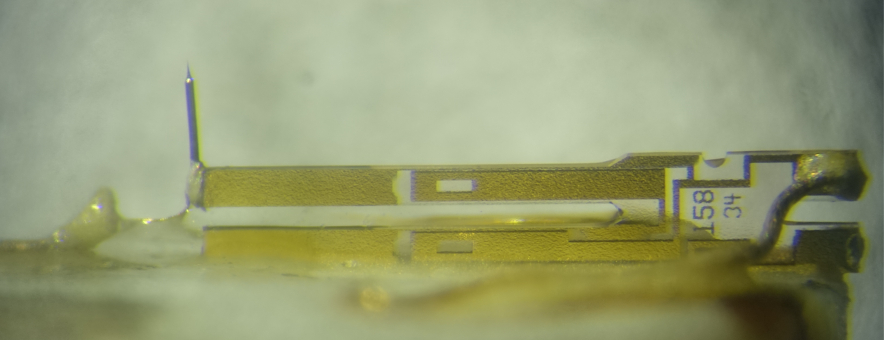
\includegraphics[width=0.6\textwidth]{./images/AFM-qplus-photograph}
		\label{fig:AFM-cantilever}}	
	\subfigure[QPlus sensor used to excite oscillations of the cantilever with controlled amplitude and frequency. Simultanious excitation of the tuning fork ($S_-$ and $S_+$) and measurement of the tunneling current ($I_t$) is possible. From \cite{AFM-qplus}]{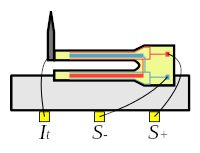
\includegraphics[width=0.3\textwidth]{./images/200px-QPlusSchematic}
		\label{fig:AFM-qplus}}
	
	\caption{Photograph \ref{fig:AFM-cantilever} and sketch \ref{fig:AFM-qplus} of AFM cantilever as used in the used setup. }
	\label{fig:AFM-tuning-fork}
\end{figure}	


\begin{figure}\centering
	\subfigure[Schematic representation of cantilever tip and atomically flat sample surface. The force between both $F_{TS}$ is indicated with an arrow. The attractive/repulsive force regimes are shown for variing tip-sample distances. From \cite{pavlicek_generation_2017}]{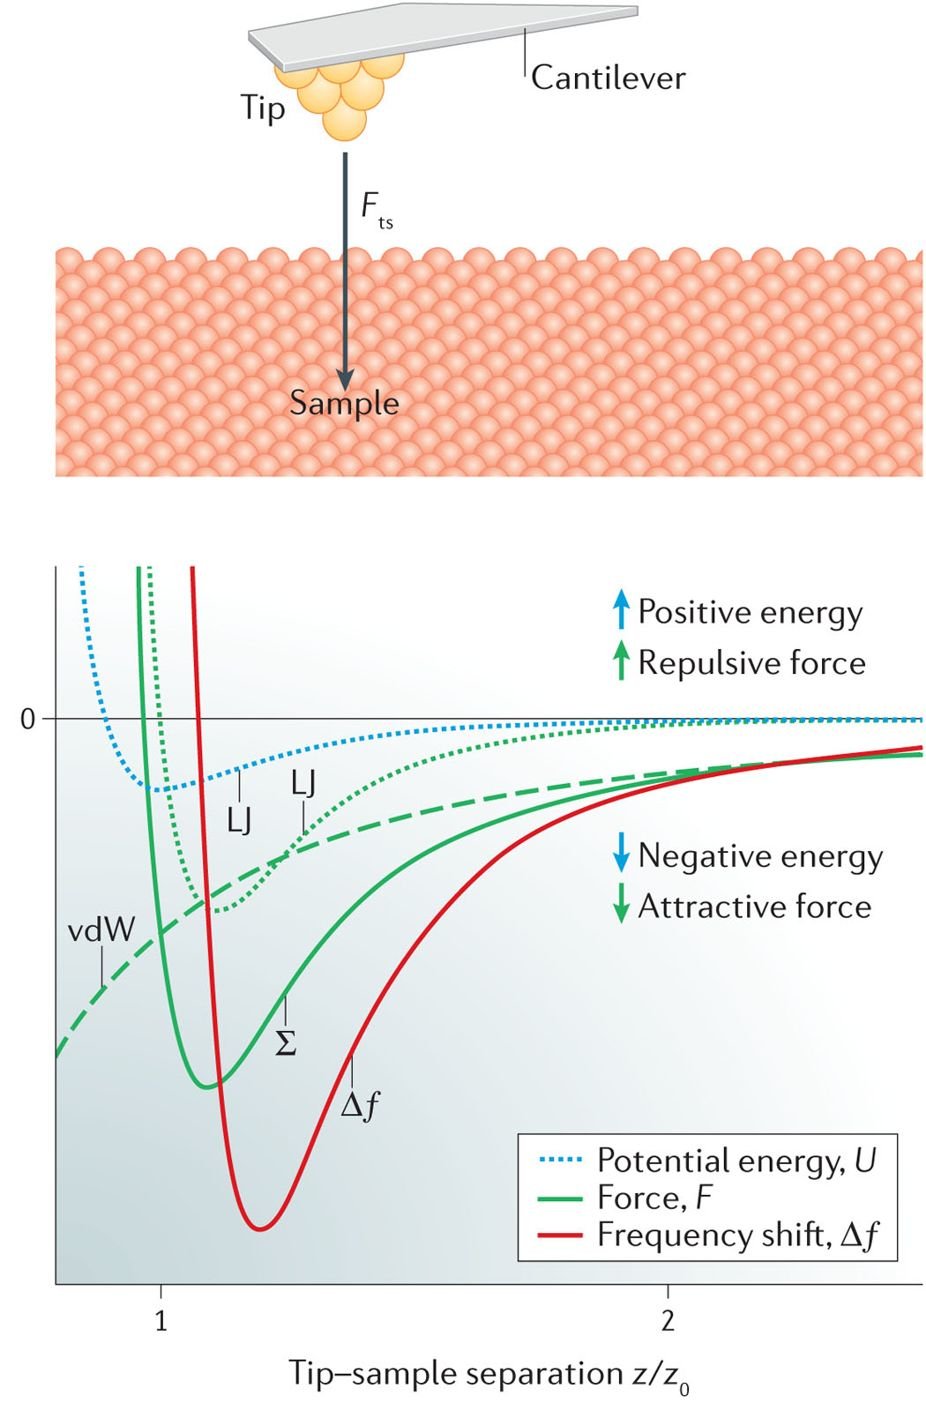
\includegraphics[width=0.6\textwidth]{./images/s41570-016-0005-f1}%
		\label{fig:AFM-force}}
	\subfigure[Enlarged sheme of AFM tip and top most sample layer. CO functionalization of the tip leads to an decreased tip apex that increases resolution. Modified from \cite{AFM-qplus}. See text for further discussion.]{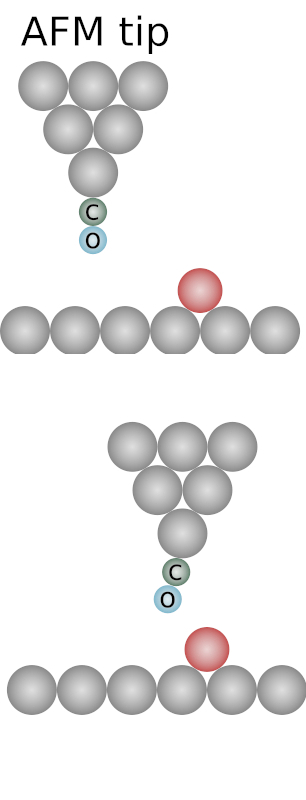
\includegraphics[width=0.3\textwidth]{./images/AFM_tip_with_CO-functionalization-mod}
		\label{fig:AFM-CO}}
	
	\caption{Basic function of a typical qplus AFM. \ref{fig:AFM-force} Sketch of tip-sample interaction together with force-distance graph. The CO functionalization of the metalic AFM tip is shown in \ref{fig:AFM-CO}}%
	\label{fig:AFM-sketch}%
\end{figure}%

When the tip moves above the surface it interacts with it due to different forces. These are typically:
\begin{itemize}
 \item van-der-waals interaction
 \item mechanical contact force
 \item capillary forces, chemical bonding, electrostatic forces, Casimir forces, solvation forces and so on
\end{itemize}

The typical resulting force between tip and sample is shown in figure \ref{fig:AFM-force}.
A magnetic tip can be used to scan for magnetic forces on the sample surface.

There are several operational modes to drive an AFM:
\begin{enumerate}
 \item \textbf{Contact (static) mode}: The cantilever is operated in contact with the sample surface. At very close proximity, repulsive forces are stronger than the attracting ones. The signal used to gain information on the sample is either the feedback loop to keep the tip at the same absolute position or directly the deflection of the cantilever.
 \item \textbf{Intermittend contact mode (tapping) mode}: While the contact mode has some disadvantages when scanning samples with an adsorbat layer (tip sticks to surface when close ehough to measure short-range forces) another mode has established. Hereby the tip oscillates with amplitudes in the \SIrange{100}{200}{\nm} regime and is not dragged the whole way across the sample. The intermittend forces acting on the tip when reaching the sample are measured. The change in amplitude when in close vicinity to the surface is a sign of the actual height.
 \item \textbf{Non-contact mode}: The cantilever is driven at its resonance frequency with amplitudes smaller than \SI{10}{\nm} and at a certain distance to the sample. Long-range forces like van-der-waals and others change the resonance frequency of the cantilever. This change is a indication of the acting force between cantilever and sample.
\end{enumerate}

\begin{itemize}
 \item AFM produces a true height-profile of the sample (and not a projection of the surface onto a 2D-map like in STM)
 \item Works in ambient pressure and even in liquids
 \item It has limited resolution especially when scanning features steeper than the tip apex
\end{itemize}

Its advantages are the comparable large image size of many hundred \si{\nm} compared to only some dozen \si{\nm} in the case of STM. Scan speeds are typically some orders of magnitude larger than those in STM so that image acquision is much faster.

To increase the resolution the tip can be functionalized with CO (see figure \ref{fig:AFM-CO}). This method is widely used \cite{kawai_multiple_2018, kawai_atomically_2015, schulz_elemental_2018, gross_chemical_2009} to investigate not only geometric features that are not accessible in STM, but also chemical differences in the sample. 